%\documentclass{article}
%\usepackage{graphicx,subfigure}
%\begin{document}

\begin{figure}[!h]
  \centering
  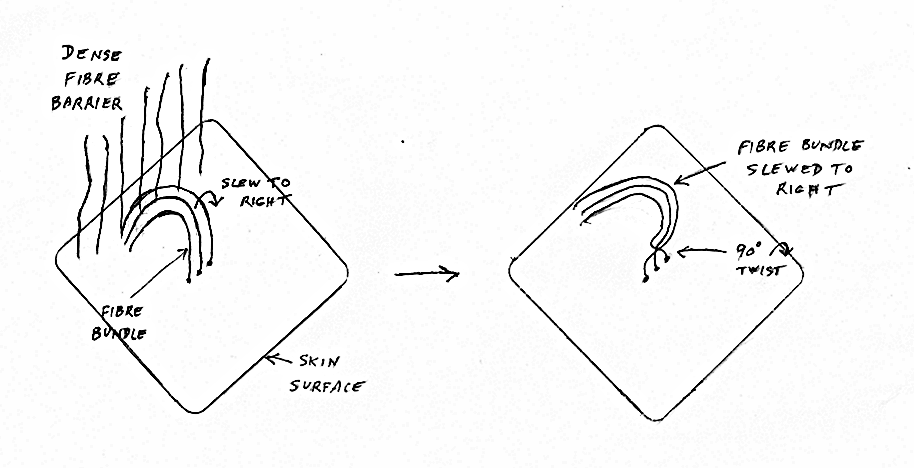
\includegraphics[width=1.1\textwidth]{fig13bfilt.png}
  \caption{A drawing showing the first loop of a growing bundle of fibres slewing to the right on encountering a dense fibre barrier in the direction of fibre curvature. A 90 degree twist occurs at the skin surface.}
  \label{twist1}
\end{figure}

%\end{document}

